\chapter{Query Language}\label{sec:specification_language}

At the heart of the \vnnlib{} standard is the \vnnlib{} query language. Heavily influenced by SMT-LIB, this language is designed as a standardised computer-readable format for expressing a wide range of satisfiability problems over neural networks. This chapter describes the syntax, scoping, typing and semantics of the query language.

\section{Syntax}
\label{sec:syntax}


Similar to SMT-LIB, the syntax of \vnnlib{} is primarily designed with the goal of machine-readability in mind. Although the syntax is somewhat human-readable, maximising readability is not a primary goal of the language. Instead it is envisaged that \vnnlib{} queries will be generated automatically by higher level tools that provide better user-orientated interfaces.

The syntax of \vnnlib{} is formally defined as Labelled Backus-Naur Form~\cite{forsberg2005labelled} (LBNF) grammar which can be found in Appendix~\ref{app:lbnf_grammar}. Instead of describing each of the production rules in detail, we will now highlight key syntactic constructs of the language via examples illustrating their usage.

Firstly, all \vnnlib{} queries are split into two parts: a list of network declarations and a list of assertions. The former allow users to specify an interface for the networks and bring new abstract variables into scope that represent the input and output values of the network. The latter than reference those variables in order to express the desired constraints that should be satisfied. Currently, the standard does not permit the interleaving of network declarations and assertions. Figure~\ref{fig:simple-query} shows an example of a simple query.

\subsection{Simple network declarations}
\label{sec:network-declarations}

 At its simplest, a network is introduced by the keyword \texttt{declare-network}, followed by a user-defined name for the network, and then declarations for its associated input and output. An input is declared using the \texttt{declare-input} keyword, followed by a variable name, its element type (e.g., \texttt{Real}, \texttt{float64}), 
and the shape of the tensor. Similarly, an output variable uses the \texttt{declare-output} keyword. In the case of Figure~\ref{fig:simple-query}, the network is named \texttt{myNetwork}, and it has one input called \texttt{X} consisting of a $1 \times 10$ tensor of real numbers and one output called \texttt{Y} consisting of a $1 \times 2$ tensor of real numbers. 
\begin{figure}[t]
    \begin{minipage}[c]{0.6\textwidth}
        \begin{lstlisting}[style=lbnf]
(declare-network myNetwork
    (declare-input  X Real [1,10])
    (declare-output Y Real [1,2])
)

(assert (>= X[0,2] 0.0))
(assert (<= X[0,2] 1.0))
(assert (<= Y[0,1] 0.5))\end{lstlisting}
    \end{minipage}%
    \begin{minipage}[c]{0.45\textwidth}
        \centering
        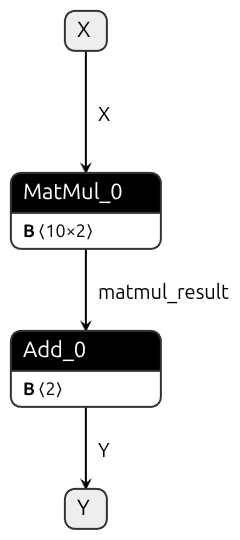
\includegraphics[height=5cm]{imgs/simple_net.onnx.png}
    \end{minipage}
    \caption{A simple \vnnlib{} specification which declares a network with a single input and output. An example of one of the many possible ONNX models compatible with this declaration is shown on the right. Note that the variable names in the declared inputs and outputs do not have to match the node names in the ONNX file.}
    \label{fig:simple-query}
\end{figure}


It is important to clarify that a network declaration only declares an \emph{interface} and by default does not refer in any way to a particular ONNX network model. When passing a query and a network to the verifier, the name of the network does not need to match the name of the ONNX model file. Instead, as described in Section~\ref{sec:verify_command}, the user will explicitly associate a network declaration to the relevant model file via the command line.
Neither do the declared names of the inputs and outputs need to match the names of the input and output nodes within the model file. This flexibility allows many different alternative ONNX models to be compatible with the same query.

All variable names follow the same syntax conventions: they are case-sensitive, must start with a letter, and may only contain letters, digits and underscores. All variable names must be unique within the query (see Section~\ref{sec:scoping_and_typing} for a more in-depth discussion). 


% The \texttt{@} character is a reserved character which is used to denote multiple applications of the same network, for the purpose of defining  hyperproperties such as monotonicity. For example \texttt{(declare-network acasXu@1 ...)} and \texttt{(declare-network acasXu@2 ...)} define two networks that are both instances of the same ONNX model,  denoted as \texttt{acasXu} in the command line interface of the verifier (See Chapter~\ref{sec:solver_interface} for more details).

\subsection{Assertions}

The second part of a \vnnlib{} query is a list of assertions that constrain the abstract tensor variables introduced by the network declarations. \vnnlib{} supports quantifier-free logical formulas as \textit{assertions}. Assertions are defined using parenthesized \texttt{(assert\ldots)} expressions, and following an SMT-LIB-like prefix syntax with the 
operator preceding its operands. An assertion is a logical formula that may include logical connectives, relational comparisons, and arithmetic expressions over declared tensors and constants.
The final satisfiability problem is then the conjunction of all the assertions.
 
\paragraph{Constants}

Numeric constant values may be referenced using basic standard integer or floating point syntax (e.g. \inlinevnn{0}, \inlinevnn{0.0}, \inlinevnn{-0.5}). 

\paragraph{Variables} 

Standard indexing notation may be used to refer to a specific element within the tensor variable. For example, Line 6 in Figure~\ref{fig:simple-query} uses \inlinevnn{X[0,2]}, to refer to the value of the element of the input tensor at row~0, column~2. All indices are zero based and currently the number of indices provided must be equal to the number of dimensions of the variable, i.e. partial indexing is not allowed.

\paragraph{Arithmetic expressions}

One forms arithmetic expressions by recursively combining constant and variable values via prefix notation. Currently the following operators are supported:
\begin{itemize}
	\item \inlinevnn{(- a)}: Negation of a term.
    \item \inlinevnn{(+ a b ...)}: Addition of two or more terms. 
    \item \inlinevnn{(* a b ...)}: Multiplication of two or more terms. 
    \item \inlinevnn{(- a b ...)}: Subtraction of two or more terms. Note that subtraction associates to the left, e.g. \inlinevnn{(- 1 2 3 4)} is the same as \inlinevnn{(- (- (- 1 2) 3) 4)} .
\end{itemize}
Arithmetic operations currently only operate over individual tensor elements and cannot be used to operate over multi-dimensional tensors (see Section~\ref{sec:scoping_and_typing} for detailed typing rules).

\paragraph{Comparisons}

The comparison operators \inlinevnn{<=}, \inlinevnn{>=}, \inlinevnn{<}, \inlinevnn{>}, \inlinevnn{=}, \inlinevnn{!=} can be used to compare the values of two arithmetic operations.
For example, \inlinevnn{(<= a b)} returns true if $a$ is less than or equal to $b$.
    
\paragraph{Boolean expressions} 

One forms boolean expressions by recursively combining comparisons via the following supported logical connectives:
\begin{itemize}
    \item \inlinevnn{(and a b ...)}: Conjunction of two or more terms.
    \item \inlinevnn{(or a b ...)}: Disjunction of two or more terms.
\end{itemize}

\subsection{More complex network declarations}
\label{sec:complex-networks-decls}

Although queries usually relate the input of a single network to its output in some way, queries can be far more complex in general. The neural network may have multiple input or output nodes, or the query may refer to intermediate hidden layers of the network or it may relate the behaviour of multiple networks. All of these use cases can be expressed within the query language.

\paragraph{Multiple input and output declarations}

Neural network that take multi-modal input or produce multi-modal output are becoming increasingly common. For example, the network in Figure~\ref{fig:multi-inputs-outputs} shows a model that takes both an image and meta-data about that image as inputs, and outputs both a bounding box around an identified object of interest and a probability distribution over the possible classs that the object belongs to. 

The query language supports such networks by allowing a network declaration to declare an arbitrary number of inputs and outputs. The question is then how is the list of declared inputs and outputs mapped to the list of inputs and outputs nodes in the ONNX model. There are two ways to specify this mapping: 
\begin{itemize}
    \item \textbf{By order:} the default is that declared inputs and outputs are mapped to the ONNX graph's inputs and outputs by matching the order of declaration in the query to the order of declaration in the ONNX model file. This is demonstrated in the top code snippet in Figure~\ref{fig:multi-inputs-outputs}
    \item \textbf{By name:} alternatively, variables can be explicitly mapped using the names of the nodes within the ONNX graph. If this method is used, all input and output variables within that network declaration must be given an explicit ONNX node name. This is demonstrated in the bottom code snippet in Figure~\ref{fig:multi-inputs-outputs}.
\end{itemize}

\begin{figure}[h!]
    \centering
    \begin{lstlisting}[style=lbnf]
(declare-network multi_io_net
    (declare-input  image    Real [1,3,224,224])
    (declare-input  metadata Real [1,10])
    (declare-output logits   Real [1,1000])
    (declare-output bbox     Real [1 4])
)\end{lstlisting}

    \begin{lstlisting}[style=lbnf]
(declare-network multi_io_net
    (declare-input  image    Real [1,3,224,224] "image_in")
    (declare-input  metadata Real [1,10] "metadata_in")
    (declare-output logits   Real [1,1000] "logits_out")
    (declare-output bbox     Real [1,4] "bbox_out")
)\end{lstlisting}

    \vspace{0.5cm}
    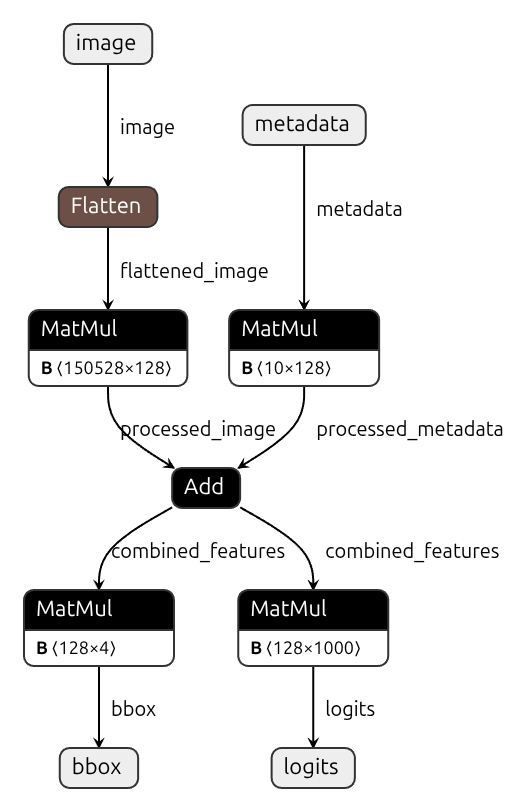
\includegraphics[height=10cm]{imgs/multi_io_net.onnx.png}
    \caption{A network with multiple inputs/outputs, mapped by declaration order.}
    \label{fig:multi-inputs-outputs}
\end{figure}


\paragraph{Hidden Node Declarations}
\label{sec:hidden-node-declarations}

In some use cases it is desirable to constrain the result of intermediate computation at the output of hidden nodes within the network. For example, when reasoning about the encodings in an encoder-decoder architecture or when reasoning about attention mechanisms.
This can be achieved by declaring hidden nodes is declared using the \texttt{declare-hidden} keyword. This declaration includes a variable name for use within the \vnnlib{} specification, 
its element type, its tensor shape, and crucially, a string identifier that specifies the corresponding node name in the ONNX graph.  Multiple
hidden nodes can be trivially declared within a single network declaration. Figure~\ref{fig:hidden-node} shows a \vnnlib{} network declaration with a hidden node.

\mnote{Talk about node names vs node output names}

\begin{figure}[h!]
    \begin{minipage}[c]{0.65\textwidth}
        \begin{lstlisting}[style=lbnf]   
(declare-network encoder
    (declare-input X Real [1,28,28])
    (declare-hidden Z Real [1,128] "encoder_output")
    (declare-output Y Real [1,10])
)\end{lstlisting}
    \end{minipage}%
    \begin{minipage}[c]{0.35\textwidth}
        \centering
        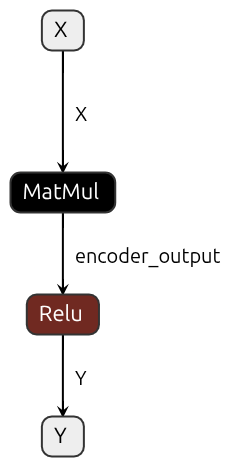
\includegraphics[height=6cm]{imgs/encoder_net.onnx.png}
    \end{minipage}
    \caption{\vnnlib{} network declaration that declares a hidden node}
    \label{fig:hidden-node}
\end{figure}

\paragraph{Multiple networks}

Often you may want to relate the behaviour of one neural network to that of another. Classic examples include: teacher-student networks where you try to train a smaller, more efficient network to mimic the output of the larger network, or observer-controller architectures.

\vnnlib{} supports defining multiple networks in by including multiple \inlinevnn{(declare-network ...)} expressions in the same query. Figure~\ref{fig:multiple-networks} 
shows an example which declares two networks representing a teacher and a student network.

\begin{figure}[h!]
    \begin{minipage}[c]{0.6\textwidth}
        \begin{lstlisting}[style=lbnf]
(declare-network teacher
    (declare-input tX Real [1,32])
    (declare-output tY Real [1,2])
)

(declare-network student
    (declare-input sX Real [1,32])
    (declare-output sY Real [1,2])
)\end{lstlisting}
    \end{minipage}
    \begin{minipage}[c]{0.4\textwidth}
        \centering
        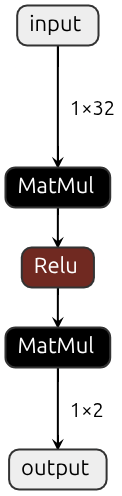
\includegraphics[height=5cm]{imgs/teacher_net.onnx.png}
        \vspace{0.5cm} 
        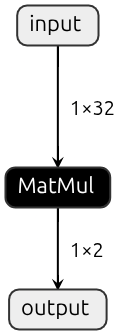
\includegraphics[height=5cm]{imgs/student_net.onnx.png}
    \end{minipage}
    \caption{Two networks declared in \vnnlib{}: \texttt{teacher\_net} and \texttt{student\_net}.}
    \label{fig:multiple-networks}
\end{figure}


\subsection{Comments and whitespace}

Comments in \vnnlib{} are denoted by a semicolon (\texttt{;}) and extend to the end of the line. They are used for annotation, explaining logic, or providing additional context. Whitespace in \vnnlib{} is used to separate tokens and improve readability. It can include spaces, tabs, and newlines. Whitespace is ignored by the parser, except where it is necessary to separate tokens.


\section{Scoping and Typing}
\label{sec:scoping_and_typing}

\mnote{TODO: Ann Roy}

\begin{itemize}
\item Unique variable names
\item Well-scoped indices within tensor dimensions
\item Inputs/hidden/output declarations in order.
\end{itemize}


\section{Semantics}
\label{sec:semantics}

\mnote{TODO: Ann Roy}


\section{Logics}
\label{sec:query_categories}

The \textit{logic} heirarchy of \vnnlib{} is a classification of the logics used to 
express a query, such as the mathematical theories, the arithmetic complexities, 
and the different semantic structures. This heirarchy is aimed at providing a clear understanding 
of the different capabilities that may be supported by verification tools. The heirarchy 
is expressed in Figure~\ref{fig:vnnlib_capabilities}.

\subsection{Neural Network Verification Queries}

Inputs and outputs of operators are \emph{tensors}, i.e.,
multidimensional arrays over some domain, usually numerical. 
If we let $\mathbb{D}$ be any such domain, a $k$-dimensional 
tensor on $\mathbb{D}$ is denoted as $x \in \mathbb{D}^{n_1 
	\times \ldots \times n_k}$.
For example, a vector of $n$ real numbers is a 1-dimensional
tensor $x \in \mathbb{R}^n$, whereas a matrix of $n \times n$ 
Booleans is a 2-dimensional tensor $x \in \mathbb{B}^{n 
	\times n}$ with $\mathbb{B} = \{0, 1\}$. A specific element 
of a tensor can be singled-out via \emph{subscripting}. 

Given a $k$-dimensional tensor $x \in \mathbb{D}^{n_1 \times 
	\ldots \times n_k}$, the element $x_{i_1, \ldots, i_k} \in 
	\mathbb{D}$ is a scalar corresponding to the indexes 
${i_1, \ldots, i_k}$. For example, in a vector of real numbers 
$x \in \mathbb{R}^n$, $x_1$ is the first element, $x_2$ the second 
and so on. In a matrix of Boleans $x \in \mathbb{B}^{n \times
  n}$, $x_{1,1}$ is the first element of the first row, $x_{2,1}$ 
is the first element of the second and so on.

An \emph{operator} $f$ is a function on tensors 
$f: \mathbb{D}^{n_{1} \times n_h} \to \mathbb{D}^{m_{1} \times m_k}$
where $h$ is the dimension of the input tensor and $k$ is the 
dimension of the output tensor. Given a set $F = \{f_1, \ldots, 
	f_p\}$ of $p$ operators, a \emph{feedforward neural network}
is a function $\nu = f_p(f_{p-1}(\ldots f_2(f_1(x))\ldots))$ obtained
through the composition of the operators in $F$ assuming that the 
dimensions of their inputs and outputs are \emph{compatible}, i.e.,
if the  output of $f_i$ is a $k$-dimensional tensor, then the input
of $f_{i+1}$ is also a $k$-dimensional tensor, for all $1 \leq i < p$.

Given a neural network $\nu : \mathbb{D}^{n_{1} \times n_h} \to
\mathbb{D}^{m_{1} \times m_k}$ built on the set of operators $\{f_1,
\ldots, f_p\}$, let $x \in \mathbb{D}^{n_{1} \times n_h}$ denote
the input of $\nu$ and $y_1, \ldots, y_p$ denote the outputs of the
operators $f_1, \ldots, f_p$ --- therefore $y_p$ is also the output
$y$ of $\nu$. We assume that, in general, a \emph{query} is a quantifier-free
first order formula $P(x, y_1, \ldots y_p)$ which should be satisfied given 
$\nu$.

More formally, given $p$ bounded sets $X_1, \ldots, X_p$ in $I$ 
such that $\Pi = \bigcup_{i=1}^p X_i$ and $s$ bounded sets $Y_1, 
\ldots, Y_s$ in $O$ such that $\Sigma = \bigcup_{i=1}^s Y_i$, we wish
to prove that  
\begin{equation}
	\label{eq:verif}
	\forall x \in \Pi \rightarrow \nu(x) \in \Sigma.
\end{equation}

The definition of the query given in equation (\ref{eq:verif})
consists of a \textit{pre-}condition $x \in \Pi$ and a 
\textit{post-}condition $\nu(x) \in \Sigma$. The 
\textit{pre-}condition encodes the bounds of the input space, i.e.,
bounds the variables that are fed to the network, and the 
\textit{post-}condition defines the safe zone, outside which the 
verification task fails.

\usetikzlibrary{
    arrows.meta,    % For arrow styles
    positioning,    % For relative positioning of nodes (e.g., below=of)
    shapes.geometric, % For shapes like rounded rectangles
    trees           % For drawing tree structures
}

\tikzset{
    % Style for the logic identifiers - reduced padding and height
    logic/.style={
        draw, 
        thick, 
        rectangle, 
        rounded corners=2pt, 
        fill=blue!10, 
        align=center, 
        minimum height=2.3em, %<-- Reduced height
        inner sep=3pt,       %<-- Reduced internal padding
        font=\small\ttfamily
    },
    % Style for the main category titles
    category/.style={
        font=\bfseries,
        align=center
    },
    % Style for the connecting arrows
    arrow/.style={
        ->,
        thick,
        >=Stealth
    }
}

\begin{figure}
    \centering
    
    % This command scales the content to the text width, maintaining aspect ratio
    \resizebox{\textwidth}{!}{%
        \begin{tikzpicture}[
            node distance=1cm and 1cm % Vertical and horizontal spacing
        ]
    
        % --- Define the four main category titles in a 2x2 grid ---
        
        % --- TOP ROW ---
        \node (theories_title) [category] at (0,0) {Theories};
        \node (arch_title)     [category] at (8,0) {Architecture};
        
        % --- BOTTOM ROW ---
        \node (arith_title)    [category] at (0,-7cm) {Arithmetic Complexity};
        \node (ortho_title)    [category] at (8,-7cm) {Orthogonal Logic};

        % --- Draw the tree for Theories (Flowing UP) ---
        \node (float_cat) [logic, below=of theories_title, xshift=1.5cm]  {FP};
        \node (f16)       [logic, below=of float_cat, xshift=-1.2cm] {FP16};
        \node (f32)       [logic, below=of float_cat, xshift=1.2cm] {FP32};
        \node (real)      [logic, left=of float_cat] {R};
        % Arrows
        \draw[arrow] (f16.north) -- (float_cat.south);
        \draw[arrow] (f32.north) -- (float_cat.south);

        % --- Draw the tree for Architecture (Flowing UP) ---
        \node (csp) [logic, below=of arch_title] {[CSP] (Constraint Satisfaction)};
        \node (fra) [logic, below=of csp]  {[FRA] (Forward Reachability)};
        % Arrow
        \draw [arrow] (fra) -- (csp);

        % --- Draw the tree for Arithmetic Complexity (Flowing UP) ---
        \node (poly)     [logic, below=of arith_title] {POLY};
        \node (linear)   [logic, below=of poly] {LINEAR};
        \node (bounds)   [logic, below=of linear]   {BOUNDS};
        % Arrows
        \draw [arrow] (bounds) -- (linear);
        \draw [arrow] (linear) -- (poly);

        % --- Draw the tree for Orthogonal Logic ---
        \node (strict) [logic, below=of ortho_title] {SI (Strict Inequality)};
        
        \end{tikzpicture}
    }%
    \caption{The \vnnlib{} Capability Hierarchy}
    \label{fig:vnnlib_capabilities}
\end{figure}

\subsection{Verifier Architecture}\label{sec:arch}

\subsubsection*{Constraint Satisfaction Problems (CSP)}\label{sec:csp}
In the context of neural network verification, a Constraint Satisfaction Problem (CSP) is a mathematical problem 
defined by a set of variables, their corresponding domains, and a set of constraints. The variables may represent
the network's inputs, hidden neuron activations, and outputs. The domains specify the possible values for these 
variables, such as an input perturbation range. The constraints encode the network's architecture, including 
transformations applied by each layer, activation functions, and the constraints imposed by the verification query itself.

The verification task is then to find an assignment of values to all variables that is both complete 
(all variables are assigned) and consistent (all constraints are satisfied). If such a solution exists, 
it represents a satisfying assignment for the query. 

\subsubsection*{Forward Reachability Analysis (FRA)}\label{sec:fra}
Forward Reachability Analysis (FRA) is a verification technique that computes an over-approximation 
of the set of all possible outputs of a neural network given a set of inputs. Formally, for a network $\nu$ 
and an input set $\Pi$, FRA aims to compute a set $\mathcal{R}$ such that the true set of all reachable outputs, 
$\nu(\Pi) = \{\nu(x) | x \in \Pi\}$, is a subset of $\mathcal{R}$. The verification property, 
$\forall x \in \Pi \rightarrow \nu(x) \in \Sigma$, is proven to be true if the computed reachable set $\mathcal{R}$ 
is entirely contained within the safe output set $\Sigma$, i.e., $\mathcal{R} \subseteq \Sigma$.

This method propagates the input set layer by layer through the network. Since computing the exact reachable set is often 
intractable, especially for networks with non-linear activation functions, FRA employs over-approximation techniques. 
These techniques use geometric shapes like hyper-rectangles (interval arithmetic), zonotopes, star sets, or polyhedra to represent 
the set of neuron activations at each layer. While computationally more efficient than exact methods, these over-approximations 
can lead to the "wrapping effect," where the computed set $\mathcal{R}$ is larger than the true reachable set, potentially causing 
the verification to fail even if the property holds, and leading to an UNKNOWN result (see Section~\ref{sec:verify_command}).

Another limitation of FRA is that it does not provide a way to encode properties that contain both pre- and post-conditions, As such, 
FRA is considered a subset of the more general Constraint Satisfaction Problem (CSP) approach, which encodes all variables and constraints 
in a single satisfiability problem.

\subsection{Theories}

\subsubsection*{Floating Point Arithmetic (FP)}
Floating-point arithmetic is a computational model that uses a finite number of bits to approximate real numbers, as standardized by IEEE 754. 
In neural network verification, this theory acknowledges that the network's weights, biases, and activations are subject to rounding errors 
after each operation. These small, cumulative errors can lead to behaviors not predicted by idealized mathematical models. For instance, due to 
the non-associativity of floating-point addition, the order of operations can affect the final output.

Verification under the theory of floating-point arithmetic is therefore crucial for providing guarantees about the actual behavior of a neural 
network deployed on physical hardware. Verification tools must soundly model these finite-precision effects by tracking the propagation of rounding errors. 
This ensures that the verification result is robust to the discrepancies between the mathematical ideal and the practical implementation.

\subsubsection*{Real Arithmetic (R)}
Real arithmetic serves as an idealized mathematical representation for neural network verification, where all numerical values and computations are 
assumed to have infinite precision. Under this theory, numbers are treated as true real numbers, and operations like addition and multiplication 
are perfectly associative and distributive, with no rounding or approximation errors. This abstraction simplifies the formal analysis of a neural 
network's properties, allowing verifiers to reason about the network's behavior without the complexities of hardware-specific implementations.

However, due to the accumulation of numerical errors in real-world neural network inference (which is done on finite-precision floating-point arithmetic), 
the guarantees obtained from verification under this theory may not directly transfer to a network's deployment. 

\subsection{Arithmetic Complexity}

\subsubsection*{Polynomial Complexity}
Polynomial complexity in neural network verification arises when the relationships between variables in the verification problem can be expressed as polynomial inequalities. 
This occurs when when the \vnnlib{} involves polynomial arithmetic expressions of the network's nodes. Verifying properties of such networks involves solving systems of polynomial constraints.

\subsubsection*{Linear Complexity}
Linear complexity pertains to verification problems where the arithmetic formulae of the query are limited to linear equations. In the case of CSP problems, the verification task can be reduced 
to checking linear inequalities, which can be efficiently solved using linear programming techniques such as MILP (Mixed Integer Linear Programming). For FRA problems, linear complexity allows 
for the use of linear over-approximations of the reachable sets, such as hyper-rectangles or zonotopes, to represent the activations of neurons in the network.

\subsubsection*{Bounds}
The most fundamental level of arithmetic complexity is the bounds logic, which deals with verifying properties that can be expressed as simple inequalities that bound the values of the network's 
inputs, outputs, or hidden nodes. In the case of FRA, input bounds are propagated through the network to determine the range of possible values for each neuron.

\subsection{Orthogonal Logic}

\subsubsection*{Strict Inequality}
The use of strict inequalities (e.g., $y > c$) in a verification property introduces specific formal and computational challenges. While non-strict inequalities ($\ge$) define closed sets, 
strict inequalities define open sets. In verification, this distinction is critical, especially at decision boundaries. To prove a property like $\forall x \in \Pi, \nu(x) > c$, the verifier 
must show that the output can never be equal to $c$.
